\documentclass[a4paper, 12pt]{article}

\usepackage{/Users/zhengz/Desktop/Math/Workspace/Homework1/homework}
%%%%%%%%%%%%%%%%%%%%%%%%%%%%%%%%%%%%%%%%%%%%%%%%%%%%%%%%%%%%%%%%%%%%%%%%%%%%%%%%%%%%%%%%%%%%%%%%%%%%%%%%%%%%%%%%%%%%%%%%%%%%%%%%%%%%%%%%
\begin{document}
%Header-Make sure you update this information!!!!
\noindent
%%%%%%%%%%%%%%%%%%%%%%%%%%%%%%%%%%%%%%%%%%%%%%%%%%%%%%%%%%%%%%%%%%%%%%%%%%%%%%%%%%%%%%%%%%%%%%%%%%%%%%%%%%%%%%%%%%%%%%%%%%%%%%%%%%%%%%%%
\large\textbf{Zhengdong Zhang} \hfill \textbf{Homework 1}   \\
Email: zhengz@uoregon.edu \hfill ID: 952091294 \\
\normalsize Course: MATH 636 - Algebraic Topology III \hfill Term: Spring 2025\\
Instructor: Dr.Daniel Dugger \hfill Due Date: $11^{th}$ April, 2025 \\
\noindent\rule{7in}{2.8pt}
\setstretch{1.1}

%%%%%%%%%%%%%%%%%%%%%%%%%%%%%%%%%%%%%%%%%%%%%%%%%%%%%%%%%%%%%%%%%%%%%%%%%%%%%%%%%%%%%%%%%%%%%%%%%%%%%%%%%%%%%%%%%%%%%%%%%%%%%%%%%%%%%%%%
%Probelm 1 
%%%%%%%%%%%%%%%%%%%%%%%%%%%%%%%%%%%%%%%%%%%%%%%%%%%%%%%%%%%%%%%%%%%%%%%%%%%%%%%%%%%%%%%%%%%%%%%%%%%%%%%%%%%%%%%%%%%%%%%%%%%%%%%%%%%%%%%%
\begin{problem}{1}
Compute the cohomology groups of the following spaces \(X\) by writing down the explicit cochain complexes (e.g. cellular cochain complexes) and computing the cohomology directly. 
In each case, compute both \(H^*(X)\) and \(H^*(X;\mathbb{Z}/2)\).
\begin{enumerate}[(a)]
\item \(S^n\)
\item The genus \(g\) torus
\item \(\mathbb{R}P^n\) and \(\mathbb{C}P^n\)
\item The space \(\mathbb{R}P^n\#\cdots \mathbb{R}P^n\) (\(g\) copies)
\end{enumerate}
\end{problem}
\begin{solution}
\begin{enumerate}[(a)]
\item When \(n=0\), \(S^0\) is the disjoint union of two points. So the cochain complex \(C^*(S^0;\mathbb{Z})\) is given by 
\[0\rightarrow \hom(\mathbb{Z}^2,\mathbb{Z})\rightarrow 0\]
Note that \(\hom(\mathbb{Z}^2,\mathbb{Z})\cong \mathbb{Z}^2\), so we have \(H^0(S^0)=\mathbb{Z}^2\) and all other cohomology groups vanishes. Similarly, we have \(H^0(S^0;\mathbb{Z}/2)=(\mathbb{Z}/2)^2\) and all other cohomology groups of coefficient \(\mathbb{Z}/2\) are zero. 
For \(n\geq 1\), consider the cellular chain complex of \(S^n\) with only one \(0\)-cell and one \(n\)-cell.
\[0\rightarrow \mathbb{Z}\rightarrow\cdots\rightarrow \mathbb{Z}\rightarrow 0\]
All boundary maps are zero. Apply the functor \(\hom(-,\mathbb{Z})\) and we get the cochain complex 
\[0\rightarrow \mathbb{Z}\rightarrow\cdots\rightarrow \mathbb{Z}\rightarrow 0\]
Similarly, apply \(\hom(-,\mathbb{Z}/2)\) and we get the cochain complex with coefficient \(\mathbb{Z}/2\)
\[0\rightarrow \mathbb{Z}/2\rightarrow\cdots\rightarrow \mathbb{Z}/2\rightarrow 0\]
So the cohomology groups for \(S^n\) \((n\geq 1)\) can be summarized as follows 
\begin{multicols}{2}
\noindent
\[H^i(S^n)=\begin{cases}
	\mathbb{Z},&\iif i=0,n;\\ 
	0,&\otherwise.
\end{cases}\]
\noindent
\[H^i(S^n;\mathbb{Z}/2)=\begin{cases}
	\mathbb{Z}/2,&\iif i=0,n;\\ 
	0,&\otherwise.
\end{cases}\]
\end{multicols}
\item Let \(X\) be the genus \(g\) torus. Consider the standard cellular structure on \(X\) with one \(0\)-cell, \(2g\) \(1\)-cells and one \(2\)-cells. The chain complex is given by 
\[0\rightarrow \mathbb{Z}\xrightarrow{0}\mathbb{Z}^{2g}\xrightarrow{0}\mathbb{Z}\rightarrow 0\]
Apply \(\hom(-,\mathbb{Z})\) and \(\hom(-,\mathbb{Z}/2)\) respectively and we have the following cochain complexes 
\[0\rightarrow \mathbb{Z}\xrightarrow{0}\mathbb{Z}^{2g}\xrightarrow{0}\mathbb{Z}\rightarrow 0\]
\[0\rightarrow \mathbb{Z}/2\xrightarrow{0}(\mathbb{Z}/2)^{2g}\xrightarrow{0}\mathbb{Z}/2\rightarrow 0\]
So the cohomology groups of \(X\) can be summarized as follows 
\begin{multicols}{2}
\noindent
\[H^i(X)=\begin{cases}
	\mathbb{Z},&\iif i=0,2;\\ 
	\mathbb{Z}^{2g},&\iif i=1;\\ 
	0,&\otherwise.
\end{cases}\]
\noindent
\[H^i(X;\mathbb{Z}/2)=\begin{cases}
	\mathbb{Z}/2,&\iif i=0,2;\\ 
	(\mathbb{Z}/2)^{2g}&\iif i=1;\\ 
	0,&\otherwise.
\end{cases}\]
\end{multicols}
\item Consider the standard cellular structure on \(\mathbb{C}P^n\) with one cell in each even dimension from \(0\) to \(2n\). The chain complex is given by 
\[0\rightarrow \mathbb{Z}\rightarrow 0\rightarrow \mathbb{Z}\rightarrow \cdots\rightarrow \mathbb{Z}\rightarrow 0\]
All boundary maps are zero. Apply \(\hom(-,\mathbb{Z})\) and \(\hom(-,\mathbb{Z}/2)\) respectively, we have cochain complexes 
\[0\rightarrow \mathbb{Z}\rightarrow 0\rightarrow \mathbb{Z}\rightarrow \cdots\rightarrow \mathbb{Z}\rightarrow 0\]
\[0\rightarrow \mathbb{Z}/2\rightarrow 0\rightarrow \mathbb{Z}/2\rightarrow \cdots\rightarrow \mathbb{Z}/2\rightarrow 0\]
So the cohomology groups of \(\mathbb{C}P^n\) can be summarized as follows 
\[H^i(\mathbb{C}P^n)=\begin{cases}
	\mathbb{Z},&\iif 0\leq i\leq 2n\ \ \text{and}\ \ i\ \ \text{even};\\ 
	0,&\otherwise.
\end{cases}\]
\[H^i(\mathbb{C}P^n;\mathbb{Z}/2)=\begin{cases}
	\mathbb{Z}/2,&\iif 0\leq i\leq 2n\ \ \text{and}\ \ i\ \ \text{even};\\ 
	0,&\otherwise.
\end{cases}\]

Consider the standard cellular structure on \(\mathbb{R}P^n\) with one cell in each dimension from \(0\) to \(n\). The chain complex is given by 
\[0\rightarrow \mathbb{Z}\xrightarrow{2}\mathbb{Z}\xrightarrow{0}\cdots\xrightarrow{2}\mathbb{Z}\xrightarrow{0}\mathbb{Z}\rightarrow 0,\ \ n\ \ \text{even}\]
\[0\rightarrow \mathbb{Z}\xrightarrow{0}\mathbb{Z}\xrightarrow{2}\cdots\xrightarrow{2}\mathbb{Z}\xrightarrow{0}\mathbb{Z}\rightarrow 0,\ \ n\ \ \text{odd}\]
Apply \(\hom(-,\mathbb{Z}/2)\), and all boundary maps become \(0\). Both odd and even cases give us the same cochain complex 
\[0\rightarrow \mathbb{Z}/2\xrightarrow{0}\cdots\xrightarrow{0}\mathbb{Z}/2\rightarrow 0\]
So the cohomology groups with coefficient \(\mathbb{Z}/2\) are given by 
\[H^i(\mathbb{R}P^n;\mathbb{Z}/2)=\begin{cases}
	\mathbb{Z}/2,&\iif i=0,1,\ldots,n;\\ 
	0,&\otherwise.
\end{cases}\]
Next, apply \(\hom(-,\mathbb{Z})\) to the chain complexes and we get 
\[0\leftarrow \mathbb{Z}\xleftarrow{2}\mathbb{Z}\xleftarrow{0}\cdots\xleftarrow{2}\mathbb{Z}\xleftarrow{0}\mathbb{Z}\leftarrow 0,\ \ n\ \ \text{even}\]
\[0\leftarrow \mathbb{Z}\xleftarrow{0}\mathbb{Z}\xleftarrow{2}\cdots\xleftarrow{2}\mathbb{Z}\xleftarrow{0}\mathbb{Z}\leftarrow 0,\ \ n\ \ \text{odd}\]
So the cohomology groups of \(\mathbb{R}P^n\) can be summarized as follows 
\[H^i(\mathbb{R}P^n)=\begin{cases}
	\mathbb{Z},&\iif i=0;\\ 
	\mathbb{Z}/2,&\iif 1\leq i\leq n-1\ \ \text{and}\ \ i\ \ \text{even};\\ 
	0,&\iif 1\leq i\leq n-1\ \ \text{and}\ \ i\ \ \text{odd};\\
	\mathbb{Z}/2,&\iif i=n\ \ \text{even};\\ 
	\mathbb{Z},& \iif i=n\ \ \text{odd};\\ 
	0,&\otherwise.
\end{cases}\]
\item Let \(X\) be the connected sum of \(g\) copies of \(\mathbb{R}P^2\). Consider the standard cellular structure on \(X\) with one \(0\)-cell, \(g\) \(1\)-cells and one \(2\)-cell. The chain complex is given by 
\[0\rightarrow \mathbb{Z}\xrightarrow{d_2}\mathbb{Z}^g\xrightarrow{0}\mathbb{Z}\rightarrow 0\]
The boundary map \(d_2\) is given by a matrix \(\begin{pmatrix}
	2\\ 
	\vdots\\ 
	2
\end{pmatrix}\). Apply \(\hom(-,\mathbb{Z}/2)\) and the coboundary map becomes \(0\), so the cochain complex with coefficient \(\mathbb{Z}/2\) is given by 
\[0\leftarrow \mathbb{Z}/2\xleftarrow{0}(\mathbb{Z}/2)^g\xleftarrow{0}\mathbb{Z}/2\leftarrow 0\]
The cohomology groups of \(X\) with coefficient \(\mathbb{Z}/2\) are 
\[H^i(X;\mathbb{Z}/2)=\begin{cases}
	\mathbb{Z}/2,&\iif i=0,2;\\ 
	(\mathbb{Z}/2)^g,&\iif i=1;\\ 
	0,&\otherwise.
\end{cases}\]
Next, apply the functor \(\hom(-,\mathbb{Z})\) and we get the cochain complex 
\[0\leftarrow \mathbb{Z}\xleftarrow{\delta_1}\mathbb{Z}^g\xleftarrow{0}\mathbb{Z}\leftarrow 0\]
where \(\delta_1\) is given by the row matrix \(\begin{pmatrix}
	2&\cdots &2
\end{pmatrix}\). So the image of \(\delta_1\) in \(\mathbb{Z}\) is \(2 \mathbb{Z}\) and \(\ker \delta_1=\mathbb{Z}^{g-1}\). The cohomology groups 
\[H^i(X)=\begin{cases}
	\mathbb{Z},&\iif i=0;\\ 
    \mathbb{Z}^{g-1},&\iif i=1;\\
	\mathbb{Z}/2,&\iif i=2;\\ 
	0,&\otherwise.
\end{cases}\]
\end{enumerate}
\end{solution}

\noindent\rule{7in}{2.8pt}
%%%%%%%%%%%%%%%%%%%%%%%%%%%%%%%%%%%%%%%%%%%%%%%%%%%%%%%%%%%%%%%%%%%%%%%%%%%%%%%%%%%%%%%%%%%%%%%%%%%%%%%%%%%%%%%%%%%%%%%%%%%%%%%%%%%%%%%%
%Probelm 2
%%%%%%%%%%%%%%%%%%%%%%%%%%%%%%%%%%%%%%%%%%%%%%%%%%%%%%%%%%%%%%%%%%%%%%%%%%%%%%%%%%%%%%%%%%%%%%%%%%%%%%%%%%%%%%%%%%%%%%%%%%%%%%%%%%%%%%%%
\begin{problem}{2}
The picture below shows a \(\Delta\)-complex \(X\) (note that \(X\cong \mathbb{R}P^2\)). Note that there are two 0-simplices \(X\) and \(Y\), three \(1\)-simplices \(a,b\) and \(c\) and two \(2\)-simplices \(P\) and \(Q\). 
\[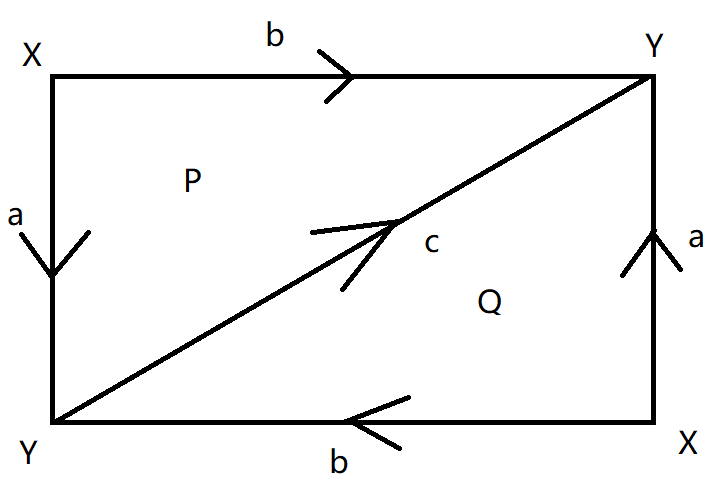
\includegraphics[scale=0.5]{Pictures/HW1-2.png}\]
Write \(\hat{X},\hat{Y}\) for the basis of \(C^0(X;\mathbb{Z})\) that is dual to \(X,Y\), and similarly for \(\hat{a},\hat{b},\hat{c}\in C^1(X;\mathbb{Z})\) and \(\hat{P},\hat{Q}\in C^2(X;\mathbb{Z})\). In this problem we will 
also work with \(C^*(X;\mathbb{Z}/2)\), and \(\hat{P}\) could denote either the cochain in \(C^2(X;\mathbb{Z})\) or in \(C^2(X;\mathbb{Z}/2)\).
\begin{enumerate}[(a)]
\item Is \(\hat{a}+\hat{b}+\hat{c}\) a cocyle? What about \(\hat{a}+\hat{c}\) and \(\hat{a}+\hat{b}\)?
\item Are the answers to (a) different in \(C^*(X; \mathbb{Z}/2)\)?
\item Cellular cohomology readily shows that \(H^1(\mathbb{R}P^2)=0\), so \(H^1(X)=0\). This means that the cocyle you found in (a) is a coboundary. Find a \(0\)-cochain \(\sigma\) such that \(\delta(\sigma)\) is your cocycle. 
\item Is \(\hat{P}\) a coboundary? What about \(\hat{P}+\hat{Q}\) and \(\hat{P}+3\hat{Q}\)?
\item Is it true that \([\hat{P}]=[\hat{Q}]\) in \(H^2(X)\)?
\item Find a \(1\)-cocycle that generates \(H^1(X;\mathbb{Z}/2)\). 
\item We have the subspace \(S^1\subseteq X\) consisting of the \(1\)-cells \(a\) and \(b\). We can restrict \(\hat{a}\) and \(\hat{b}\) to this \(S^1\), and we will call those by the same name. Complete the following 
\[[p\hat{a}+q\hat{b}]=0\ \text{in}\ H^1(S^1)\ \ \text{if and only if}\underline{\hspace{4cm}}\]
\item Analyze the map \(H^1(X;\mathbb{Z}/2)\rightarrow H^1(S^1;\mathbb{Z}/2)\). Is it injective? Surjective?
\item Given a cochain \(\alpha\in C^1(X;\mathbb{Z}/2)=\hom(C_1(X),\mathbb{Z}/2)\) and a chain \(v\in C_1(X)\) we can evaluate \(\alpha\) on \(v\) to get an element \(\alpha(v)\in \mathbb{Z}/2\). True or false: If \(v=[b]+[c]\) 
then for all cocycles \(\alpha,\alpha'\in C^1(X;\mathbb{Z}/2)\) such that \([\alpha]=[\alpha']\) in \(H^1(X;\mathbb{Z}/2)\) we have \(\alpha(v)=\alpha'(v)\). 
\item Re-do the previous part if \(v=[b]-[a]\). 
\item If \([\alpha]=[\alpha']\) in \(H^1(X;\mathbb{Z}/2)\) then \(\alpha-\alpha'=\delta(\beta)\) for some \(\beta\in C^0(X;\mathbb{Z}/2)\). What would you need to know about \(v\) in order to show that \(\alpha(v)=\alpha'(v)\), no matter what \(\beta\) is?
\end{enumerate}
\end{problem}
\begin{solution}
\begin{enumerate}[(a)]
\item Let \(\partial\) be the differential in the chain complex and \(\delta\) be the codifferential in the cochain complex. We can calculate by definition 
\[\delta(\hat{a}+\hat{b}+\hat{c})(P)=(\hat{a}+\hat{b}+\hat{c})(\partial P)=(\hat{a}+\hat{b}+\hat{c})(a+c-b)=1\]
This implies \(\delta(\hat{a}+\hat{b}+\hat{c})\) is not the zero map, so it is not a cocycle. Similarly, we have 
\[\delta(\hat{a}+\hat{c})(P)=(\hat{a}+\hat{c})(a+c-b)=2\]
So \(\hat{a}+\hat{c}\) is not a cocycle. For \(\hat{a}+\hat{b}\), we have 
\[\delta(\hat{a}+\hat{b})(P)=(\hat{a}+\hat{b})(a+c-b)=0\]
\[\delta(\hat{a}+\hat{b})(Q)=(\hat{a}+\hat{b})(b+c-a)=0\]
We know all the \(2\)-chains are generated by \(P\) and \(Q\), so this implies \(\delta(\hat{a}+\hat{b})=0\) for all \(2\)-chains. Thus, \(\hat{a}+\hat{b}\) is a cocycle. 
\item Now we take the coefficient to be \(\mathbb{Z}/2\). \(\hat{a}+\hat{b}\) is still a cocycle and \(\hat{a}+\hat{b}+\hat{c}\) is still not a cocycle by the same calculation. For \(\hat{a}+\hat{c}\), we have 
\[\delta(\hat{a}+\hat{c})(P)=(\hat{a}+\hat{c})(a+c-b)=0\]
\[\delta(\hat{a}+\hat{c})(Q)=(\hat{a}+\hat{c})(b+c-a)=0\]
So in this case, \(\hat{a}+\hat{c}\) becomes a cocycle. 
\item Suppose we have a 0-cochain \(m\hat{X}+n\hat{Y}\) satisfying \(\delta(m\hat{X}+n\hat{Y})=\hat{a}+\hat{b}\). Then we have 
\begin{align*}
	\delta(m\hat{X}+n\hat{Y})(a)&=(m\hat{X}+n\hat{Y})(Y-X)=n-m=1,\\ 
	\delta(m\hat{X}+n\hat{Y})(b)&=(m\hat{X}+n\hat{Y})(Y-X)=n-m=1,\\ 
	\delta(m\hat{X}+n\hat{Y})(c)&=(m\hat{X}+n\hat{Y})(Y-Y)=0.
\end{align*}
We can choose \(n=1\) and \(m=0\) as a solution. So \(\delta(\hat{Y})=\hat{a}+\hat{b}\).
\item Suppose there is a \(1\)-cochain \(k\hat{a}+m\hat{b}+n\hat{c}\) satisfying \(\delta(k\hat{a}+m\hat{b}+n\hat{c})=\hat{P}\). Then we have 
\begin{align*}
	\delta(k\hat{a}+m\hat{b}+n\hat{c})(P)&=(k\hat{a}+m\hat{b}+n\hat{c})(a+c-b)=k+n-m=1,\\ 
	\delta(k\hat{a}+m\hat{b}+n\hat{c})(Q)&=(k\hat{a}+m\hat{b}+n\hat{c})(b+c-a)=n+m-k=0.
\end{align*}
Combine two equations together and we have \(2n=1\). There is no solution in \(\mathbb{Z}\), so such a \(1\)-cochain does not exist. This implies \(\hat{P}\) is not a coboundary. Similarly, for \(\hat{P}+\hat{Q}\), we get two equations 
\begin{align*}
	k+n-m&=1,\\ 
	m+n-k&=1.
\end{align*}
Combine two equations and we get \(n=1\). So \(\hat{P}+\hat{Q}\) is a coboundary and we have \(\delta(\hat{c})=\hat{P}+\hat{Q}\). For \(\hat{P}+3\hat{Q}\), we have two equations 
\begin{align*}
	k+n-m&=1,\\ 
	m+n-k&=3.
\end{align*}
Combine two equations and we get \(n=2\). So \(\hat{P}+3\hat{Q}\) is a coboundary and we have \(\delta(\hat{b}+2\hat{c})=\hat{P}+3\hat{Q}\). 
\item This is the same as asking if \([\hat{P}-\hat{Q}]=0\) in \(H^2(X)\). Or equivalently, is \(\hat{P}-\hat{Q}\) a coboundary? Use the same notation for the previous question and write down the equations 
\begin{align*}
	k+n-m&=1,\\ 
	m+n-k&=-1.
\end{align*}
Combine two equations and we get \(n=0\). So \(\hat{P}-\hat{Q}\) is a coboundary and we have \(\delta(\hat{a})=\hat{P}-\hat{Q}\). This proves that \([\hat{P}]=[\hat{Q}]\) in \(H^2(X)\). 
\item We know \(X\cong \mathbb{R}P^2\), so \(H^1(X;\mathbb{Z}/2)\cong \mathbb{Z}/2\) is generated by a non zero element. We have calculated in (b) that \(\hat{a}+\hat{c}\) is a cocycle. We need to show that \(\hat{a}+\hat{c}\) is not a coboundary. Suppose 
\(m\hat{X}+n\hat{Y}\) is a 0-cochain such that \(\delta(m\hat{X}+n\hat{Y})=\hat{a}+\hat{c}\). Then we have 
\begin{align*}
	\delta(m\hat{X}+n\hat{Y})(a)&=(m\hat{X}+n\hat{Y})(Y-X)=1,\\ 
	\delta(m\hat{X}+n\hat{Y})(b)&=(m\hat{X}+n\hat{Y})(Y-X)=0.
\end{align*}
We have no solutions for these two equations so \(\hat{a}+\hat{c}\) is not a coboundary. This implies that \([\hat{a}+\hat{c}]\) is a nonzero element in \(H^1(X;\mathbb{Z}/2)\), so it is a generator. 
\item \([p\hat{a}+q\hat{b}]=0\) in \(H^1(S^1)\) is the same as \(p\hat{a}+q\hat{b}\) is a 1-coboundary in \(C^1(S^1)\). Suppose we have a 0-cochain \(m\hat{X}+n\hat{Y}\) such that 
\[\delta(m\hat{X}+n\hat{Y})=p\hat{a}+q\hat{b}\]
This is equivalent to 
\begin{align*}
	\delta(m\hat{X}+n\hat{Y})(a)&=(m\hat{X}+n\hat{Y})(Y-X)=m-n=p,\\ 
	\delta(m\hat{X}+n\hat{Y})(b)&=(m\hat{X}+n\hat{Y})(Y-X)=m-n=q.
\end{align*}
The two equations having solutions in \(\mathbb{Z}\) is equivalent to \(p=q\). So we can conclude that 
\[[p\hat{a}+q\hat{b}]=0\ \text{in}\ H^1(S^1)\ \ \text{if and only if}\ \ p=q\]
\item We know \(X\cong \mathbb{R}P^2\), so \(H^1(X;\mathbb{Z}/2)\cong H^1(S^1;\mathbb{Z}/2)\cong \mathbb{Z}/2\). So the map \(i^*:H^1(X;\mathbb{Z}/2)\rightarrow H^1(S^1;\mathbb{Z}/2)\) induced by the inclusion \(i:S^1\rightarrow X\) is either the zero map or 
an isomorphism. We have already shown in (f) that \(\hat{a}+\hat{c}\) is a generator of \(H^1(X;\mathbb{Z}/2)\). Note that \(S^1\) does not have \(c\) as a 1-cell, so \(i^*(\hat{a}+\hat{c})=\hat{a}\) in \(H^1(S^1;\mathbb{Z}/2)\). By (g), we know that 
\(\hat{a}\) is not a coboundary. This proves that \(i^*\) is not a zero map, so \(i^*\) is an isomorphism, which is both injective and surjective. 
\item This is false. From (a), (b), (c) and (f), we know that \(\hat{a}+\hat{c}\) and \(\hat{a}+\hat{b}\) are both cocycles in \(C^1(X;\mathbb{Z}/2)\), and \(\hat{a}+\hat{b}\) is also a coboundary. So \(\hat{a}+\hat{c}+\hat{a}+\hat{b}=\hat{b}+\hat{c}\) represents the same 
cohomology class as \(\hat{a}+\hat{c}\) in \(H^1(X;\mathbb{Z}/2)\), namely \([\hat{a}+\hat{c}]=[\hat{b}+\hat{c}]\) in \(H^1(X;\mathbb{Z}/2)\). And by calculation, we have 
\[(\hat{a}+\hat{c})(v)=(\hat{a}+\hat{c})([b]+[c])=1\]
\[(\hat{b}+\hat{c})(v)=(\hat{b}+\hat{c})([b]+[c])=0\] 
This shows the claim is false. 
\item This is true. Suppose \(\alpha,\alpha'\in C^1(X;\mathbb{Z}/2)\) are cocycles representing the same cohomology class. Then \(\alpha-\alpha'\) is a coboundary. There exists a 0-chain \(m\hat{X}+n\hat{Y}\) such that 
\(\delta(m\hat{x}+n\hat{Y})=\alpha-\alpha'\). Then for \(v=[b]-[a]\), we have 
\[\alpha(v)-\alpha'(v)=(\alpha-\alpha')([b]-[a])=\delta(m\hat{X}+n\hat{Y})([b]-[a])=(m\hat{X}+n\hat{Y})(Y-X-Y+X)=0.\]
\item We have 
\[0=\alpha(v)-\alpha'(v)=\delta(\beta)(v)=\beta(\partial v)\]
for all \(\beta\in C^0(X;\mathbb{Z}/2)\). This implies \(\partial v=0\), namely \(v\) is a coboundary in \(C^1(X)\).
\end{enumerate}
\end{solution}

\noindent\rule{7in}{2.8pt}
%%%%%%%%%%%%%%%%%%%%%%%%%%%%%%%%%%%%%%%%%%%%%%%%%%%%%%%%%%%%%%%%%%%%%%%%%%%%%%%%%%%%%%%%%%%%%%%%%%%%%%%%%%%%%%%%%%%%%%%%%%%%%%%%%%%%%%%%
%Probelm 3
%%%%%%%%%%%%%%%%%%%%%%%%%%%%%%%%%%%%%%%%%%%%%%%%%%%%%%%%%%%%%%%%%%%%%%%%%%%%%%%%%%%%%%%%%%%%%%%%%%%%%%%%%%%%%%%%%%%%%%%%%%%%%%%%%%%%%%%%
\begin{problem}{3}
For an abelian group \(B\), write \(B[0]\) for the chain complex which has \(B\) in degree zero and zeros everywhere else. Write \(\Sigma^nB[0]\) for the result of 
shifting this complex up \(n\) spots, so that it has \(B\) in degree \(n\).\\ 
Let \(C_*\) be a chain complex of abelian groups. Prove that \(\alpha\in \hom(C_n,B)\) is a cocyle in \(\hom(C_*,B)\) if and only if \(\alpha:C_*\rightarrow \Sigma^n B[0]\) is a chain map. 
Then prove that the set of chain homotopy classes of maps \([C_*,\Sigma^nB[0]]\) is in bijective correspondence with \(H^n(\hom(C_*,B))\).
\end{problem}
\begin{solution}
We divided the proof into two parts. Each part prove one claim. 
\begin{enumerate}[(a)]
\item Let \(\alpha\in \hom(C_n,B)\) be a cocycle. We define a chain map 
% https://q.uiver.app/#q=WzAsMTAsWzIsMCwiQ19uIl0sWzEsMCwiQ197bisxfSJdLFszLDAsIkNfe24tMX0iXSxbMCwwLCJcXGNkb3RzIl0sWzQsMCwiXFxjZG90cyJdLFswLDEsIlxcY2RvdHMiXSxbNCwxLCJcXGNkb3RzIl0sWzEsMSwiMCJdLFszLDEsIjAiXSxbMiwxLCJCIl0sWzAsOSwiXFxhbHBoYSIsMl0sWzEsNywiMCIsMl0sWzIsOCwiMCIsMl0sWzMsMV0sWzEsMCwiXFxwYXJ0aWFsIl0sWzAsMiwiXFxwYXJ0aWFsIl0sWzIsNF0sWzgsNl0sWzksOCwiMCIsMl0sWzcsOSwiMCIsMl0sWzUsN11d
\[\begin{tikzcd}
	\cdots & {C_{n+1}} & {C_n} & {C_{n-1}} & \cdots \\
	\cdots & 0 & B & 0 & \cdots
	\arrow[from=1-1, to=1-2]
	\arrow["\partial", from=1-2, to=1-3]
	\arrow["0"', from=1-2, to=2-2]
	\arrow["\partial", from=1-3, to=1-4]
	\arrow["\alpha"', from=1-3, to=2-3]
	\arrow[from=1-4, to=1-5]
	\arrow["0"', from=1-4, to=2-4]
	\arrow[from=2-1, to=2-2]
	\arrow["0"', from=2-2, to=2-3]
	\arrow["0"', from=2-3, to=2-4]
	\arrow[from=2-4, to=2-5]
\end{tikzcd}\]
To show that this is a well-defined chain map, we only need to check the commutativity of the two squares above. Recall that \(\alpha\) is a cocycle in \(\hom(C_*,B)\), so we have 
\[0=\delta \alpha=\alpha\circ \partial\]
by definition of the codifferential. This tells us the above two squares commutes. Conversely, suppose we have a well-defined chain map \(\alpha:C_*\rightarrow \Sigma^nB[0]\), then the commutativity of the square 
tells us that \(\alpha\circ \partial=0\). This is equivalent to \(\delta\alpha=0\), so \(\alpha\) viewed as a map \(\alpha:C_n\rightarrow B\) is a cocycle. 
\item From (a), we know that we can define a map 
\begin{align*}
	\phi:H^n(\hom(C_*,B))&\rightarrow [C_*,\Sigma^nB[0]],\\ 
	     [\alpha]&\mapsto [\alpha]_h
\end{align*}
where \([\alpha]\) is the cohomology class of the cocycle \(\alpha\) and \([\alpha]_h\) is the chain homotopy class of the chain map \(\alpha\). To show this map is well-defined, consider \(\alpha,\alpha'\) are two cocycles representing the same cohomology class, then 
there exists \(\beta\in \hom(C_{n-1},B)\) such that \(\delta(\beta)=\alpha-\alpha'\). Consider the following diagram 
% https://q.uiver.app/#q=WzAsMTAsWzIsMCwiQ19uIl0sWzEsMCwiQ197bisxfSJdLFszLDAsIkNfe24tMX0iXSxbMCwwLCJcXGNkb3RzIl0sWzQsMCwiXFxjZG90cyJdLFswLDEsIlxcY2RvdHMiXSxbNCwxLCJcXGNkb3RzIl0sWzEsMSwiMCJdLFszLDEsIjAiXSxbMiwxLCJCIl0sWzAsOSwiXFxhbHBoYSIsMix7Im9mZnNldCI6MX1dLFsxLDcsIjAiLDJdLFsyLDgsIjAiLDJdLFszLDFdLFsxLDAsIlxccGFydGlhbCJdLFswLDIsIlxccGFydGlhbCJdLFsyLDRdLFs4LDZdLFs5LDgsIjAiLDJdLFs3LDksIjAiLDJdLFs1LDddLFsyLDksIlxcYmV0YSIsMV0sWzAsOSwiXFxhbHBoYSciLDAseyJvZmZzZXQiOi0xfV0sWzAsNywiMCIsMV1d
\[\begin{tikzcd}
	\cdots & {C_{n+1}} & {C_n} & {C_{n-1}} & \cdots \\
	\cdots & 0 & B & 0 & \cdots
	\arrow[from=1-1, to=1-2]
	\arrow["\partial", from=1-2, to=1-3]
	\arrow["0"', from=1-2, to=2-2]
	\arrow["\partial", from=1-3, to=1-4]
	\arrow["0"{description}, from=1-3, to=2-2]
	\arrow["\alpha"', shift right, from=1-3, to=2-3]
	\arrow["{\alpha'}", shift left, from=1-3, to=2-3]
	\arrow[from=1-4, to=1-5]
	\arrow["\beta"{description}, from=1-4, to=2-3]
	\arrow["0"', from=1-4, to=2-4]
	\arrow[from=2-1, to=2-2]
	\arrow["0"', from=2-2, to=2-3]
	\arrow["0"', from=2-3, to=2-4]
	\arrow[from=2-4, to=2-5]
\end{tikzcd}\]
Note that 
\[\alpha-\alpha'=\delta(\beta)=\beta\circ \partial+0\circ 0\]
So \(\beta\) gives a chain homotopy between the chain map \(\alpha\) and \(\alpha'\). This implies \([\alpha]_h=[\alpha']_h\). Conversely, from (a), we can define a map 
\begin{align*}
	\psi:[C_*,\Sigma^nB[0]]&\rightarrow H^n(\hom(C_*,B)),\\ 
	     [\alpha]_h&\mapsto [\alpha]
\end{align*}
By the previous discussion we know that if two chain maps \(\alpha,\alpha'\) are chain homotopic, then there exists a map \(\beta:C_{n-1}\rightarrow B\) such that 
\[\beta\circ \partial +0\circ 0=\alpha-\alpha'\]
So \(\psi\) is also well-defined. It is easy to check that \(\psi\circ \phi=id\) and \(\phi\circ \psi=id\). Thus, we can conclude that \([C_*,\Sigma^nb[0]]\) is bijective to \(H^n(\hom(C_*,B))\).
\end{enumerate}
\end{solution}

\noindent\rule{7in}{2.8pt}
%%%%%%%%%%%%%%%%%%%%%%%%%%%%%%%%%%%%%%%%%%%%%%%%%%%%%%%%%%%%%%%%%%%%%%%%%%%%%%%%%%%%%%%%%%%%%%%%%%%%%%%%%%%%%%%%%%%%%%%%%%%%%%%%%%%%%%%%
%Probelm 4 
%%%%%%%%%%%%%%%%%%%%%%%%%%%%%%%%%%%%%%%%%%%%%%%%%%%%%%%%%%%%%%%%%%%%%%%%%%%%%%%%%%%%%%%%%%%%%%%%%%%%%%%%%%%%%%%%%%%%%%%%%%%%%%%%%%%%%%%%
\newpage 

\begin{problem}{4}
Consider a commutative diagram 
% https://q.uiver.app/#q=WzAsMjEsWzEsMCwiMCJdLFsyLDAsIjAiXSxbMywwLCIwIl0sWzEsMSwiQV8zIl0sWzIsMSwiQV8yIl0sWzMsMSwiQV8xIl0sWzEsMiwiQl8zIl0sWzIsMiwiQl8yIl0sWzMsMiwiQl8xIl0sWzEsMywiQ18zIl0sWzIsMywiQ18yIl0sWzMsMywiQ18xIl0sWzEsNCwiMCJdLFsyLDQsIjAiXSxbMyw0LCIwIl0sWzAsMSwiMCJdLFswLDIsIjAiXSxbMCwzLCIwIl0sWzQsMSwiMCJdLFs0LDIsIjAiXSxbNCwzLCIwIl0sWzE1LDNdLFszLDQsImRfQSJdLFs0LDUsImRfQSJdLFs1LDE4XSxbMTYsNl0sWzYsNywiZF9CIl0sWzcsOCwiZF9CIl0sWzgsMTldLFsxNyw5XSxbOSwxMCwiZF9DIl0sWzEwLDExLCJkX0MiXSxbMTEsMjBdLFswLDNdLFszLDYsImZfMyIsMl0sWzYsOSwiZ18zIiwyXSxbOSwxMl0sWzEsNF0sWzQsNywiZl8yIiwyXSxbNywxMCwiZ18yIiwyXSxbMTAsMTNdLFsyLDVdLFs1LDgsImZfMSIsMl0sWzgsMTEsImdfMSIsMl0sWzExLDE0XV0=
\[\begin{tikzcd}
	& 0 & 0 & 0 \\
	0 & {A_3} & {A_2} & {A_1} & 0 \\
	0 & {B_3} & {B_2} & {B_1} & 0 \\
	0 & {C_3} & {C_2} & {C_1} & 0 \\
	& 0 & 0 & 0
	\arrow[from=1-2, to=2-2]
	\arrow[from=1-3, to=2-3]
	\arrow[from=1-4, to=2-4]
	\arrow[from=2-1, to=2-2]
	\arrow["{d_A}", from=2-2, to=2-3]
	\arrow["{f_3}"', from=2-2, to=3-2]
	\arrow["{d_A}", from=2-3, to=2-4]
	\arrow["{f_2}"', from=2-3, to=3-3]
	\arrow[from=2-4, to=2-5]
	\arrow["{f_1}"', from=2-4, to=3-4]
	\arrow[from=3-1, to=3-2]
	\arrow["{d_B}", from=3-2, to=3-3]
	\arrow["{g_3}"', from=3-2, to=4-2]
	\arrow["{d_B}", from=3-3, to=3-4]
	\arrow["{g_2}"', from=3-3, to=4-3]
	\arrow[from=3-4, to=3-5]
	\arrow["{g_1}"', from=3-4, to=4-4]
	\arrow[from=4-1, to=4-2]
	\arrow["{d_C}", from=4-2, to=4-3]
	\arrow[from=4-2, to=5-2]
	\arrow["{d_C}", from=4-3, to=4-4]
	\arrow[from=4-3, to=5-3]
	\arrow[from=4-4, to=4-5]
	\arrow[from=4-4, to=5-4]
\end{tikzcd}\]
in which every row and every column is a chain complex. Assume that all the homology groups in each row are zero except for \(H_3(C)\). Also assume that all the homology 
groups of the columns are zero except for the kernel of the map labelled \(f_1\). Prove that \(\ker f_1\cong H_3(C)\).
\end{problem}
\begin{solution}
We first define a map \(\phi:\ker f_1\rightarrow H_3(C)\). Let \(a\in \ker f_1\), the exactness implies that \(d_A:A_2\rightarrow A_1\) is surjective, so there exists \(a'\in A_2\) such that \(d_A(a')=a\). We know 
that \(f_2(a')\in B_2\) and by commutativity of the square we have 
\[d_B(f_2(a'))=f_1(d_A(a'))=f_1(a)=0\]
since \(a\in \ker f_1\). This implies \(f_2(a')\in \ker d_B\) and by exactness there exists a unique \(b\in B_3\) such that \(d_B(b)=f_2(a')\). We define 
\begin{align*}
    \ker f_1&\rightarrow C_3,\\ 
     a&\mapsto g_3(b).
\end{align*} 
Note that \(d_C(g_3(b))=g_2(d_B(b))=g_2(f_2(a'))=0\) by exactness of the middle column. So we obtain a map \(\phi:\ker f_1\rightarrow H_3(C)\) because \(C_4=0\). We need to check the map is well defined.
\par
We check that the map \(\phi\) does not depend on the choice of \(a'\in A_2\). Suppose \(a',a'' \in A_2\) with \(a=d_A(a')=d_A(a'')\). Then \(a'-a''\in \ker d_A\) and by exactness, there 
exists \(c\in A_3\) such that \(d_A(c)=a'-a''\). This implies 
\[f_2(a'-a'')=f_2(d_A(c))=d_B(f_3(c))\]
Suppose \(b,b'\in B_3\) such that \(d_B(b)=f_2(a')\) and \(d_B(b')=f_2(a'')\). Then we have 
\[d_B(b-b')=f_2(a'-a'')=d_B(f_3(c))\]
Because the middle row is exact, so \(d_B\) is injective. This implies \(b-b'=f_3(c)\). Then 
\[g_3(b)-g_3(b')=g_3(f_3(c))=0\]
\par 
To see this is a group homomorphism, consider \(x,y\in C_3\), we need to show that \(\phi(x+y)=\phi(x)+\phi(y)\). Note that we can choose \(x',y',x'+y'\in A_2\) as the preimage of \(x,y,x+y\) since the choice does not matter in the final result. All other processes are completely determined by a group homomorphism, so \(\phi\) is indeed a group homomorphism. 
\par 
We define another map \(\psi:H_3(C)\rightarrow \ker f_1\). Rewrite the whole diagram in the following way 
% https://q.uiver.app/#q=WzAsMjEsWzMsMSwiQ18zIl0sWzIsMSwiQl8zIl0sWzEsMSwiQV8zIl0sWzAsMSwiMCJdLFs0LDEsIjAiXSxbMywyLCJDXzIiXSxbMywzLCJDXzEiXSxbMiwyLCJCXzIiXSxbMiwzLCJCXzEiXSxbMSwyLCJBXzIiXSxbMSwzLCJBXzEiXSxbMSwwLCIwIl0sWzIsMCwiMCJdLFszLDAsIjAiXSxbMCwyLCIwIl0sWzAsMywiMCJdLFsxLDQsIjAiXSxbNCwyLCIwIl0sWzIsNCwiMCJdLFszLDQsIjAiXSxbNCwzLCIwIl0sWzEzLDBdLFswLDUsImRfQyJdLFs1LDYsImRfQyJdLFs2LDE5XSxbMTIsMV0sWzEsNywiZF9CIl0sWzcsOCwiZF9CIl0sWzgsMThdLFsxMSwyXSxbMiw5LCJkX0EiXSxbOSwxMCwiZF9BIl0sWzEwLDE2XSxbMywyXSxbMiwxLCJmXzMiXSxbMSwwLCJnXzMiXSxbMCw0XSxbMTQsOV0sWzksNywiZl8yIl0sWzcsNSwiZ18yIl0sWzUsMTddLFsxNSwxMF0sWzEwLDgsImZfMSJdLFs4LDYsImdfMSJdLFs2LDIwXV0=
\[\begin{tikzcd}
	& 0 & 0 & 0 \\
	0 & {A_3} & {B_3} & {C_3} & 0 \\
	0 & {A_2} & {B_2} & {C_2} & 0 \\
	0 & {A_1} & {B_1} & {C_1} & 0 \\
	& 0 & 0 & 0
	\arrow[from=1-2, to=2-2]
	\arrow[from=1-3, to=2-3]
	\arrow[from=1-4, to=2-4]
	\arrow[from=2-1, to=2-2]
	\arrow["{f_3}", from=2-2, to=2-3]
	\arrow["{d_A}", from=2-2, to=3-2]
	\arrow["{g_3}", from=2-3, to=2-4]
	\arrow["{d_B}", from=2-3, to=3-3]
	\arrow[from=2-4, to=2-5]
	\arrow["{d_C}", from=2-4, to=3-4]
	\arrow[from=3-1, to=3-2]
	\arrow["{f_2}", from=3-2, to=3-3]
	\arrow["{d_A}", from=3-2, to=4-2]
	\arrow["{g_2}", from=3-3, to=3-4]
	\arrow["{d_B}", from=3-3, to=4-3]
	\arrow[from=3-4, to=3-5]
	\arrow["{d_C}", from=3-4, to=4-4]
	\arrow[from=4-1, to=4-2]
	\arrow["{f_1}", from=4-2, to=4-3]
	\arrow[from=4-2, to=5-2]
	\arrow["{g_1}", from=4-3, to=4-4]
	\arrow[from=4-3, to=5-3]
	\arrow[from=4-4, to=4-5]
	\arrow[from=4-4, to=5-4]
\end{tikzcd}\]
Note that we still have exactness everywhere except for \(C_3\) vertically and \(A_1\) horizontally. Following the same argument as above we can define a map \(\psi:H_3(C)\rightarrow \ker f_1\). By comparison with defintiion of these maps, we can see that 
\(\psi\circ \phi=id\) and \(\phi\circ \psi=id\). This proves that \(\phi\) is an isomorphism and \(\ker f_1\cong H_3(C)\).

\end{solution}

\end{document}